\documentclass[11pt]{article}

\usepackage[margin=1in]{geometry}
\usepackage{amsmath}
\usepackage{graphicx}
\usepackage{float}

\title{RL Lab 3 -- MC Prediction}
\author{Fotios Kapotos}
\date{}

\begin{document}

\maketitle

\section{Monte Carlo prediction on blackjack}

\subsection{Monte Carlo prediction}

The value function is highest when the player already has a large sum, especially when holding a usable ace. In those states the player can safely hit or stick with a good chance of finishing near 21. The value drops when the dealer shows a strong card such as 9, 10, or Ace, because the dealer is then more likely to end with a strong hand. States with small player sums are mostly negative since the player is still far from 21 and is exposed to more future risk.

\begin{figure}[H]
    \centering
    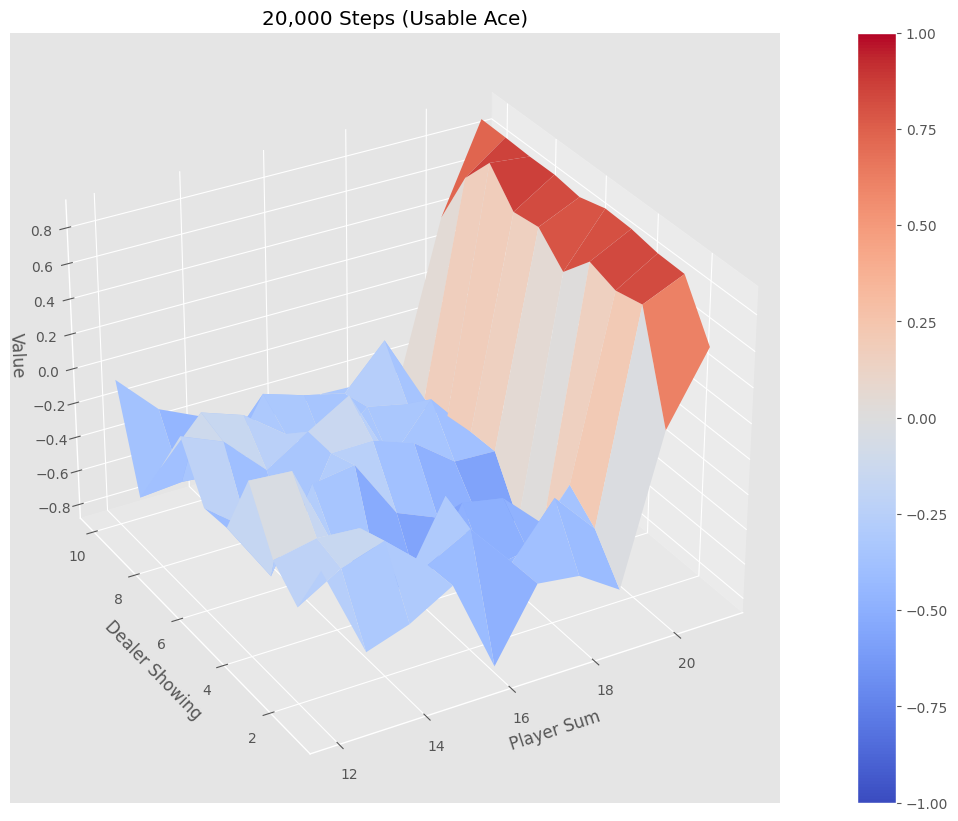
\includegraphics[width=0.48\textwidth]{figures/20000ace.png}
    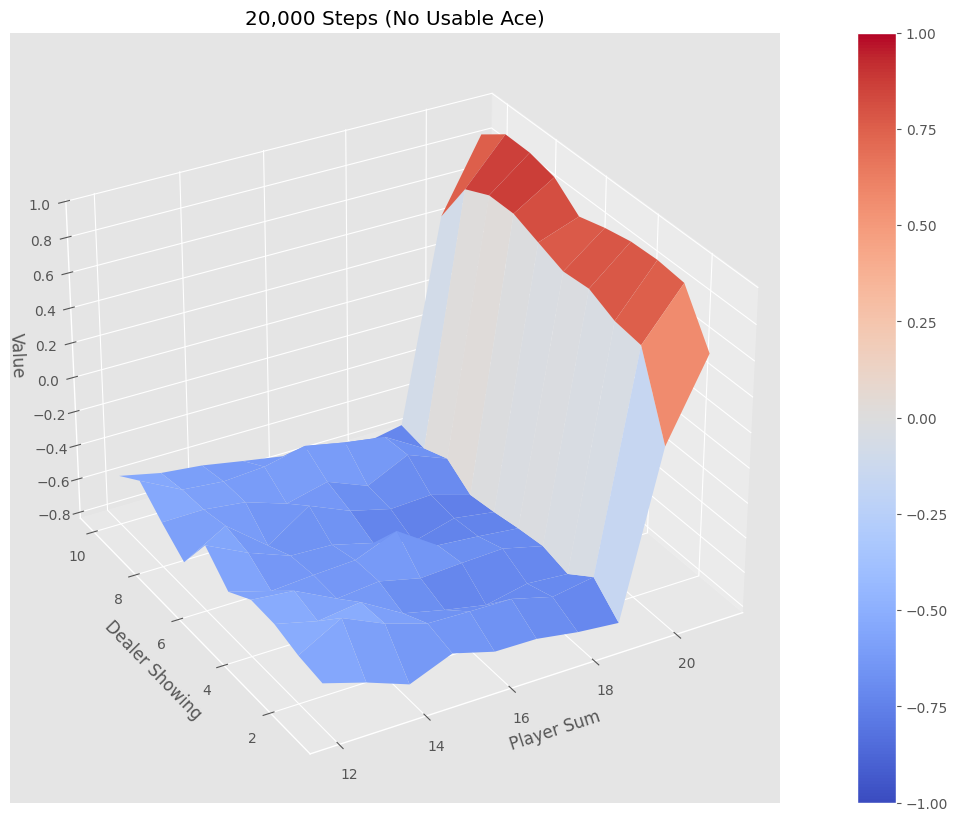
\includegraphics[width=0.48\textwidth]{figures/20000noace.png}
    \caption{Monte Carlo value estimates after 20,000 episodes.}
\end{figure}

\subsection{Monte Carlo prediction on multiple episodes}

Increasing \texttt{num\_episodes} reduces variance in the Monte Carlo estimate. With fewer episodes the learned surface is noisy and unstable because many states are visited only a small number of times. As the number of episodes grows, the value surface becomes smoother and more consistent, which indicates that the empirical returns are averaging toward the underlying expected value function.

\begin{figure}[H]
    \centering
    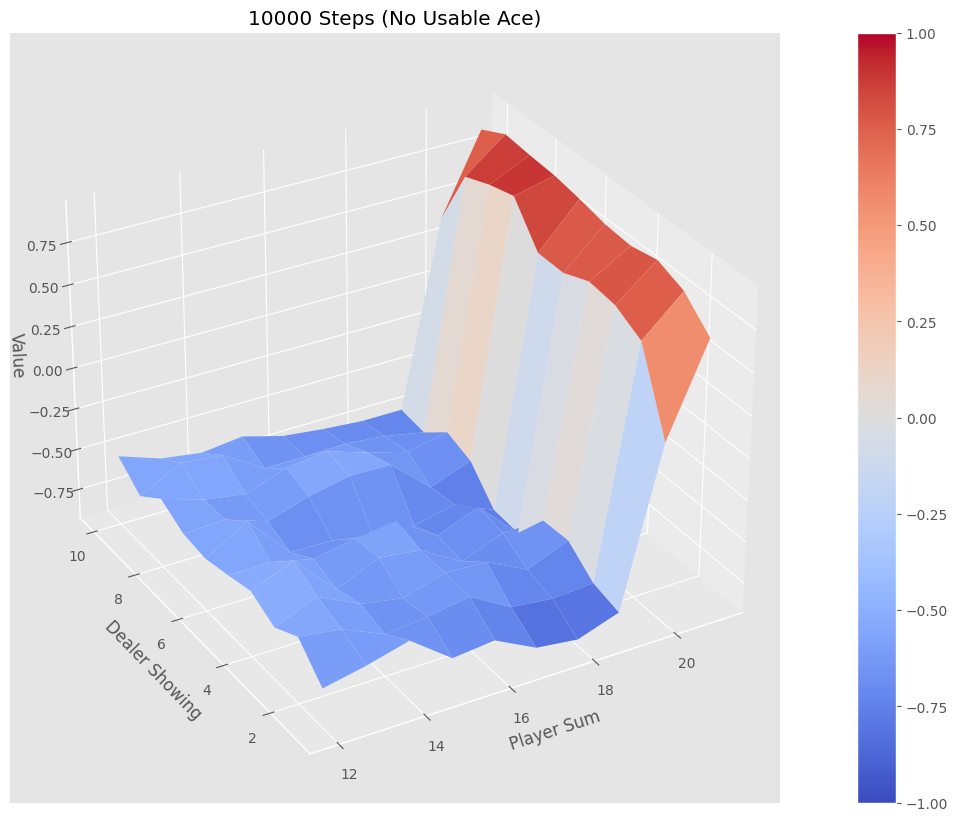
\includegraphics[width=0.48\textwidth]{figures/mc_prediction_10000_steps_no_usable_ace.png}
    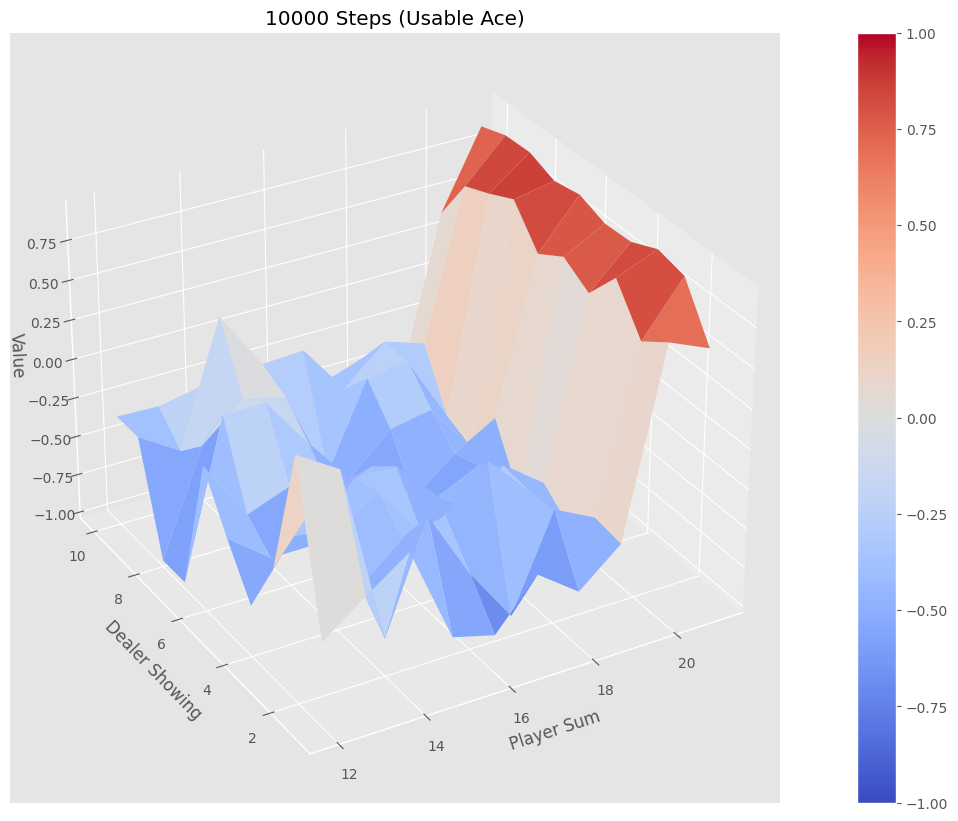
\includegraphics[width=0.48\textwidth]{figures/mc_prediction_10000_steps_usable_ace.png}

    \vspace{0.5em}

    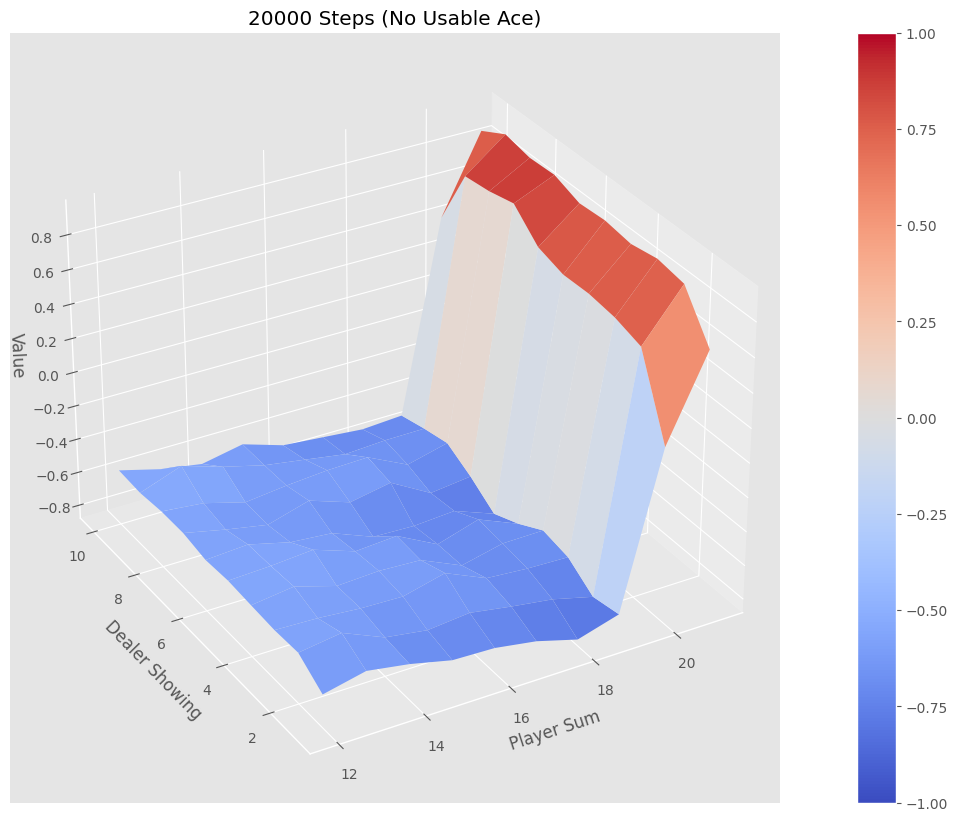
\includegraphics[width=0.48\textwidth]{figures/mc_prediction_20000_steps_no_usable_ace.png}
    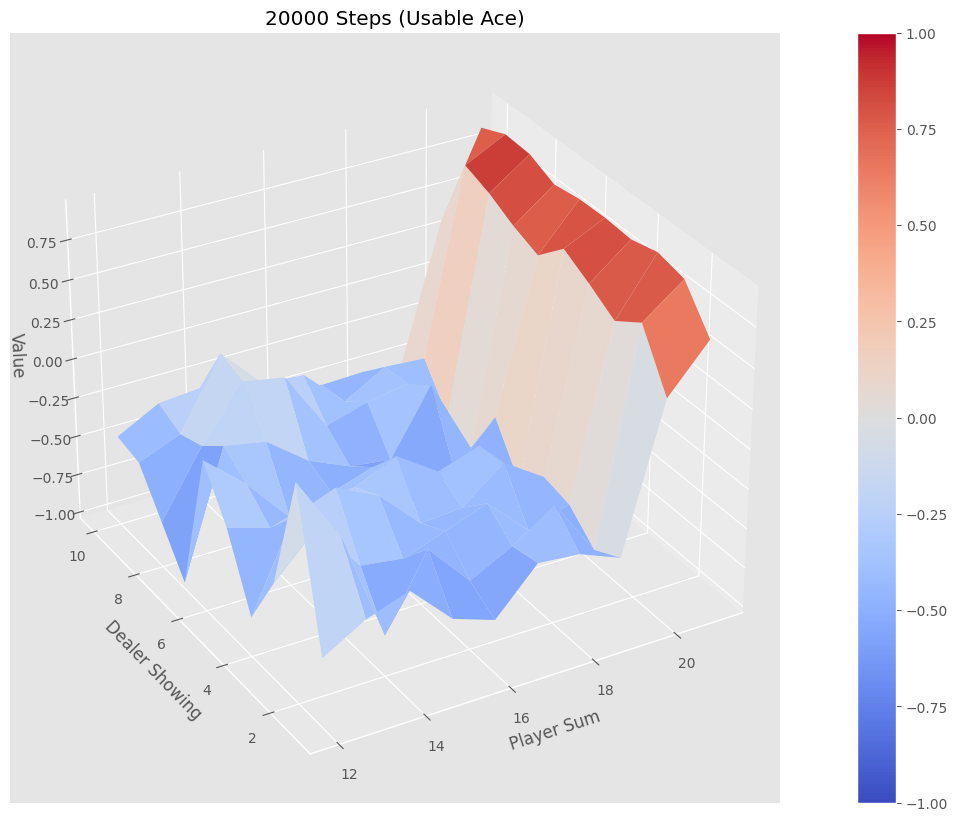
\includegraphics[width=0.48\textwidth]{figures/mc_prediction_20000_steps_usable_ace.png}
    \caption{Monte Carlo value estimates with more episodes become smoother and less noisy. Top: 10,000 episodes. Bottom: 200,000 episodes.}
\end{figure}

\section{Temporal Difference}

\begin{enumerate}

\item Comment on the effects of the number of episodes on TD's estimated value graph and interpret the results.\\
With only a few episodes, TD estimates remain close to the initial guess and the curve is still rough. As the number of episodes increases, the estimate moves steadily toward the true state values. This is exactly what we expect from TD(0): each episode refines the estimate using bootstrapped updates, so repeated experience gradually pulls the approximation toward the correct trend.

\begin{figure}[H]
    \centering
    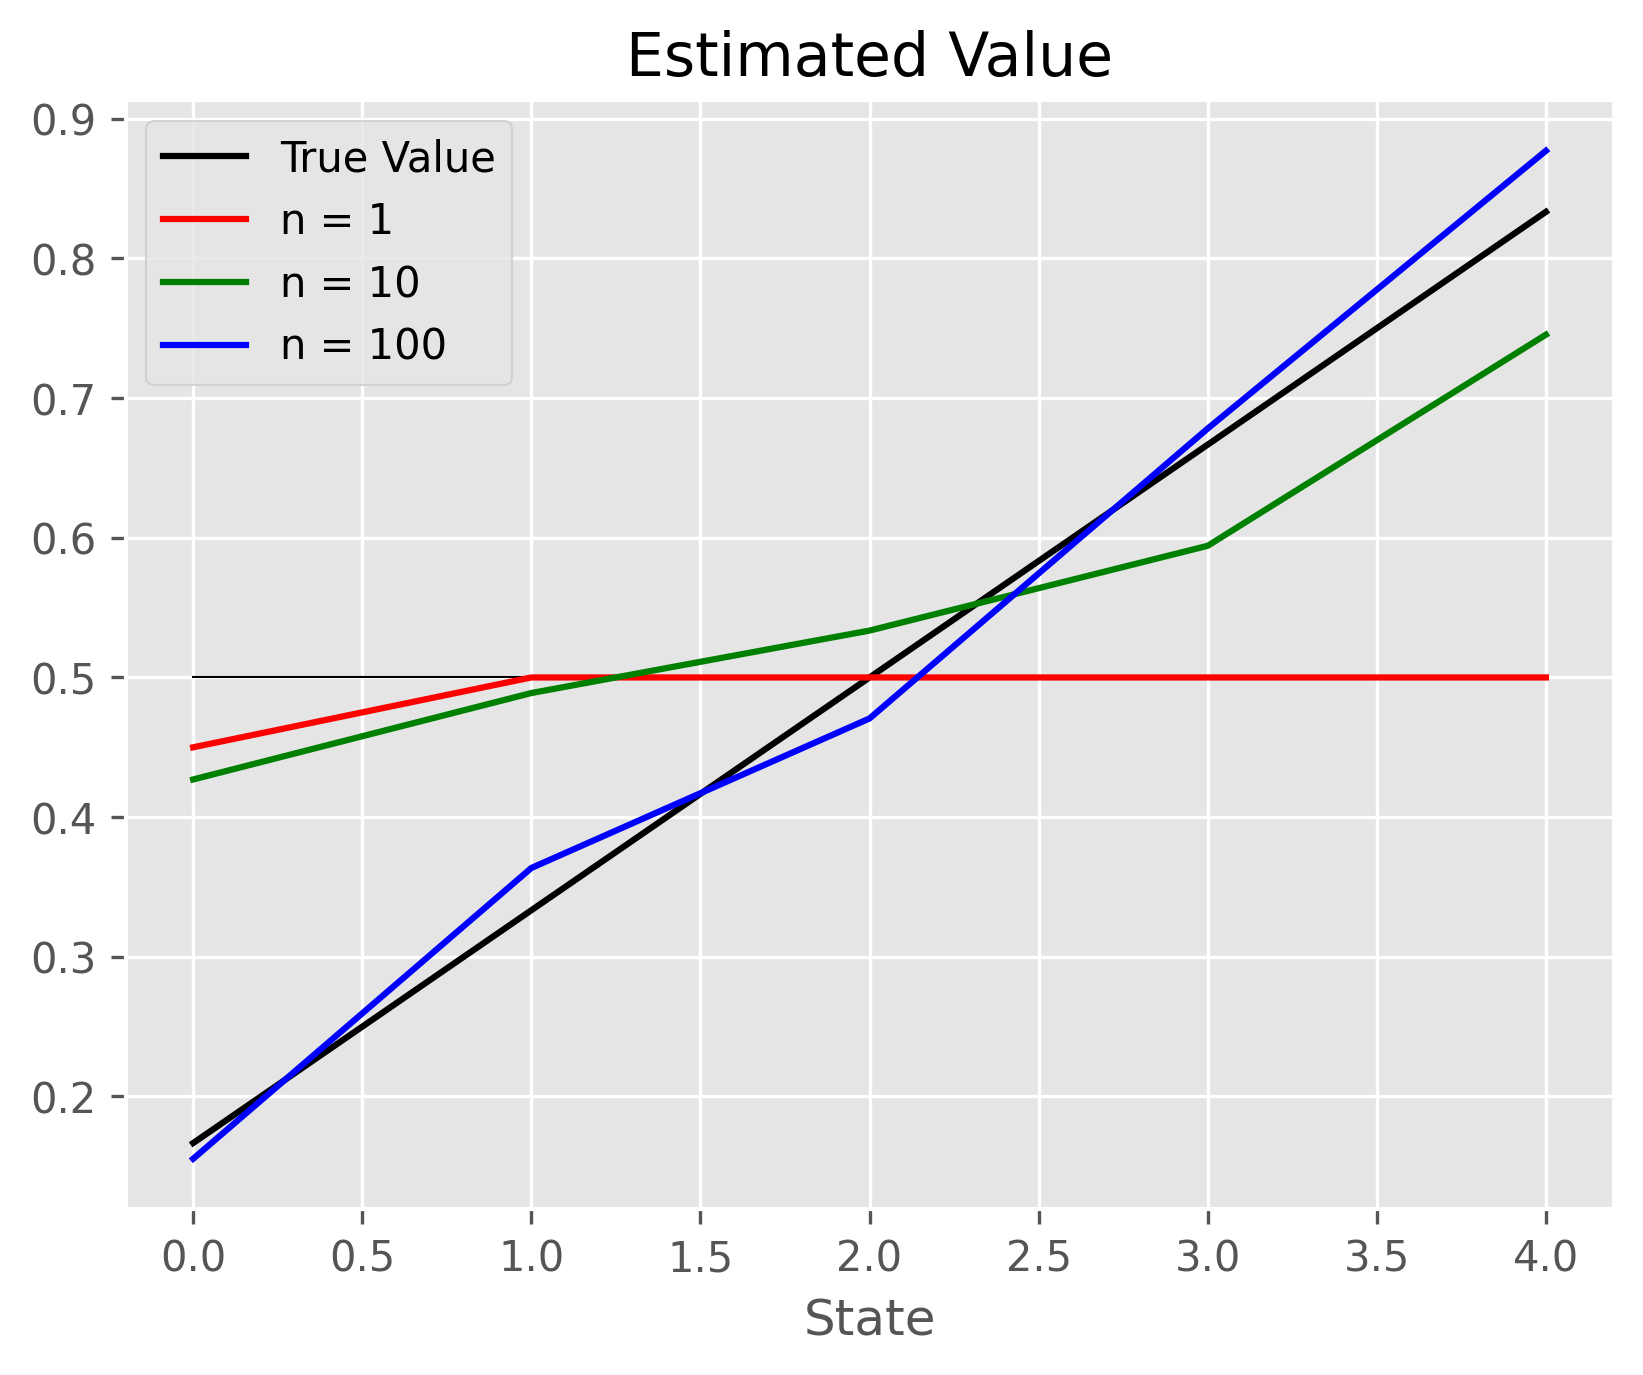
\includegraphics[width=0.7\textwidth]{figures/td_estimated_value.png}
    \caption{TD estimated values after different numbers of episodes.}
\end{figure}

\item Comment on the effects of the step size on the empirical RMS error and explain the results.  
Compare TD and MC performances and interpret, i.e., give your intuitions as to why one is outperforming the other.  
The step size controls the speed-stability tradeoff. Larger step sizes learn faster at the beginning, but they also introduce more variance and can make the error curve noisier. Smaller step sizes are more stable, but they improve more slowly.

In this experiment TD performs better than MC in the early phase: its RMS error drops faster because TD updates after every transition and bootstraps from the current estimate instead of waiting for the full return. MC uses complete returns, so its updates have higher variance and learning is slower at the start. With a suitable step size, MC can eventually become competitive, but TD is clearly more sample-efficient in the beginning.

\begin{figure}[H]
    \centering
    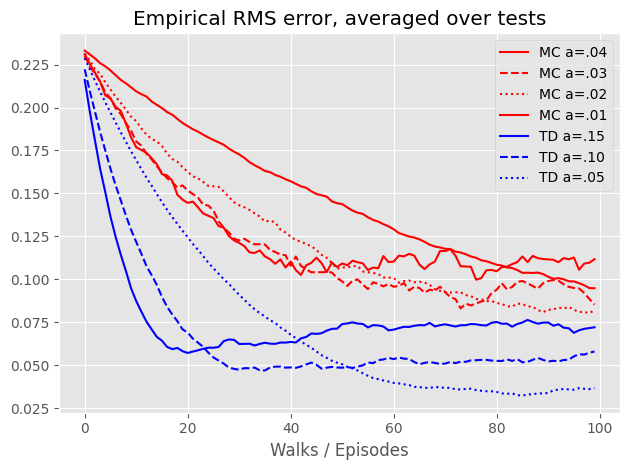
\includegraphics[width=0.7\textwidth]{figures/td_mc_rms_error.png}
    \caption{Empirical RMS error for TD and MC under different step sizes.}
\end{figure}

\end{enumerate}

\end{document}
